\section{Koncepce - elementární CA a jeho úprava}
Elementární CA je jednodimenzionální CA, ve kterém je následující stav každé
\textit{buňky} vypočítán pomocí jeho současného stavu, stavu 2
\textit{okolních buněk} a zvoleného \textit{pravidla} (IMS 209).
Buňky se můžou nacházet v 1 ze 2 stavů (0 a 1).
Pravidlem rozumíme hodnotu v rozmezí 0 až 255, která představuje
pro které kombinace buňky a jejího okolí bude výsledný stav 0 nebo 1.

Výpočet stavů následující generace můžeme vypočítat následovně (C++ "pseudokód"):
\lstinputlisting{eca.cpp}
Pro obvyklý elementární CA je použito pouze 1 pravidlo a to je aplikováno
pro každou \textit{generaci}.
Tato práce zkoumá, co se stane při aplikování různých pravidel (například
aplikování N střídajících se pravidel) pro každou generaci a v tom také
spočívá úprava elementárního CA. Je možné tedy argumentovat tím, že se již
nejedná o elementární CA, avšak jejich princip je podobný a pro jednoduchost
pochopení je tento název použit.

Mimo jiné je důležitou částí CA jeho vizualizace. K tomuto je nejvhodnější
a nejjednodušší použít 2D pole (matici), kde barva buněk představuje jejich stav,
souřadnice X jednotlivé buňky a souřadnice Y generaci.

\begin{figure}[h]
	\centering
	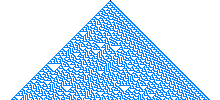
\includegraphics[width=1.0\textwidth]{rule_30.png}
	\caption{Prvních 100 generací pravidla 30 (shora dolů - 1. generace
	má černou barvu)}
\end{figure}
